% #############################################################################
%															Bahnplanung und Steuerung
% #############################################################################
\chapter{Bahnplanung und Steuerung}
\label{bahnplanung_steuerung_cha}

% ********************************************************************************
% 										Aufgabenstellung
% ********************************************************************************
\section{Aufgabenstellung}
\label{bahnplanung_aufgabenstellung_sec}
\authorsection{\editoroier}

Was die Aufgabestellung für die Bahnplanung und Steuerung betrifft, so kann man das in Abstraktionsschichten einteilen:
LowLevel-Ansteuerung, Inverse Kinematik, Bahnplanung und Kollisionsvermeidung.
Außerdem sollte man das alles auch Simulieren können.

Als Ausgangssituation hatte man die Grundlagen der Odete für die LowLevel-Ansteurung und die inverse Kinematik. Sonst waren, Bahnplanung/Steuerung und Kollisionsvermeidung zunächst nicht vorhanden. Eine Simulationsumgebung war vorhanden, es fehlte aber noch die Programmierung der Gui .

Nach dem Bottom-Up Prinzip hat man zunächst, die LowLevel-Ansteuerung von der Odete angepasst und mittels Simulation getestet.

\todo[inline]{inverse Kinematik richtig erklären, mit Diagramm} 

Das \textit{DriveAlongPath} Modul, welches sich mit der inverse Kinematik beschäftigt, dient um aus eine Trajektorie aus 3 Punkte die nötige Koordinaten für \textit{OmniDrive} zu berechnen.
Falls es sich bspw. um ein Industrieroboter handeln würde, dann würde die inverse Kinematik die nötige Gelenkwinkeleinstellungen berechnen, um mit dem Greifer eine neue Position zu erreichen.
Danach würde die inverse Dynamik die entsprechende Motor-Kräfte und Momente berechnen.

Die Bahnplanung berechnet Trajektoriepunkte auf Basis der Mensch-Position und Geschwindigkeit, welche von der Kinect-Kamera geliefert werden.
Außerdem werden hier diverse Transformationen von Welt zu Roboter bzw. Bild-Koordinaten und zurück gemacht.
Nebenbei, wird der Pfad gespeichert damit der Roboter es später alleine abfahren kann.

Zum Schluß wird eine ständige Überprüfung der geplante Trajektorie gemacht, um Kollisionen zu vermeiden.
Um Hindernisse zu umfahren, werden der A*-Algorithmus und ein Potentialfeld eingesetzt.
Letzteres wirkt, dass es \glqq teuer\grqq \space ist in der nähe von Hindernisse zu fahren.



% ********************************************************************************
% 										Grundlagen Bahnplanung
% ********************************************************************************
\section{Grundlagen der Bahnplanung und Steuerung}
\label{bahnplanung_grundlagen_sec}
\authorsection{\editoroier}

\subsection{Bahnplanung}

Bahnplanung befaßt sich mit dem Problem, eine kollisionsfreie Bahn zu finden die  ein Robotersystem
von der aktuellen Position in die Zielposition überführt. Damit gehört es zu einer der Basisprobleme der Robotik. Die Verfahren kann man nach unterschiedliche Gesichtspunkte klassifizieren \cite{rob1}.

Nach Robotertyp:
\begin{itemize}
\item Bahnplanung für Manipulatoren (Schweißen bei Industrierobotern z.B.)
\item Bahnplanung für mobile Roboter
\item Bahnplanung für Laufmaschinen und anthropomorphe Systeme
\item Greif- und Montageplanung
\end{itemize}

Nach dem Zustandsraum wo die Planung stattfindet:
\begin{itemize}
\item Gelenkwinkelzustandsraum (Konfigurationsraum, der Raum alle möglichen Gelenkwinkelkonfigurationen des Roboters )
\item Euklidischer Raum (Arbeitsraum, 3D / 6D)
\item Sensorzustandsraum
\item Objektzustandsraum
\end{itemize}

Nach Vollständigkeit:
\begin{itemize}
\item Vollständige Verfahren (liefern immer eine Korrekte Lösung und können ermitteln ob keine Lösung existiert)
\item Probabilistisch Vollständige Verfahren (Falls eine Lösung existiert konvergiert die Wahrscheinlichkeit, dass eine Lösung gefunden wird, bei fortschreitender Zeit gegen 1. Existiert keine Lösung, kann dies nicht ermittelt werden
)
\end{itemize}

Nach Navigationsart:
\begin{itemize}
\item Globale Pfadplanung bedeutet, eine Trajektorie zum Ziel zu planen wenn dem Roboter eine Karte der Umgebung bevorliegt und er sich dort lokalisieren kann.
\item Lokale Pfadplanung wird eingesetzt um Hindernisse zu umfahren und wird bei mobilen Robotern meist in Konbination mit einem globalen Planer benutzt. 
\end{itemize}

Weil die explizite Berechnung des kollisionsfreien Konfigurationsraum bei Roboter mit mehr Freiheitsgrade als 3 sehr teuer ist, benutzt man oft den impliziten Konfigurationsraum. D. h., dass die Bahnplanung in Konfigurationsraum stattfindet, aber die Kollisionen und Abstände in Arbeitsraum berechnet werden und ins diskretisierte Konfigurationsraum transformiert \citep{innoKonz}. So wird der Konfigurationsraum während der Suche exploriert.

Der Ablauf eines Planungsverfahren ist normalerweise in zwei geteilt.
\begin{enumerate}
\item Eine Roadmap oder Graph aufbauen mittels \gls{Voronoi}, \gls{Sichtgraphen}, \gls{Zellenzerlegung} oder zufällige Knoten je nach Sampling Strategie(für \gls{PRM} Verfahren z.B.).
\item Im Graph ein Weg von Startknoten zum Zielknoten finden mittels A*-Algorithmus oder andere Suchalgorithmen für Graphen.
\end{enumerate}

\subsection{Steuerung}

Weil die gefundene Trajektorie normalerweise nicht glatt ist werden für die Steuerung unterschiedliche Interpolationsarten verwendet. Die Bahnsteuerung kann in Kartesischen Raum oder im Konfigurationsraum stattfinden. In Kartesischen Raum ist es näher an der zu lösenden Aufgabe, man muss dann aber für jeden Punkt die inverse Kinematik berechnen. Die Steuerung in Konfigurationsraum hingegen liegt näher an den Gelenken, dafür ist die Formulierung der Trajektorie umständlicher. Vor und Nachteile beider Optionen kann man auf der Tabelle \ref{fig:steurungProContra} sehen.


\begin{table}[h]
		\centering
		\begin{tabular}{| p{7cm} | p{7cm}|}
\hline
\textbf{Kartesischer Raum} & \textbf{Konfigurationsraum}\\
\hline
+ Bahn einfacher zu formulieren & + Ansteuerung der Gelenke ist
einfacher\\
+ Interpolation ist einfacher & + Trajektorie ist eindeutig und
berücksichtigt Grenzen\\

- Inverse Kinematik ist für jeden Trajektorienpunkt zu lösen & - Interpolation für mehrere
Gelenke\\
- Geplante Trajektorie nicht immer ausführbar & - Formulierung der Trajektorie umständlicher\\
\hline
		\end{tabular}
		\caption{\label{fig:steurungProContra} Vor und Nachteile der Steuerung im Kartesischen und Konfigurationsraum Quelle: \citep{rob1}}
		\end{table}	
Es gibt unterschiedliche Interpolationsarten:  Zirkular, Linear und Spline-Bahn oder auch approximative Bahnsteuerung.
Bei der Linearinterpolation wird einfach zwischen zwei Teiltrajektorien interpoliert wie man auf der Abbildung \ref{fig:linearinterpolation} sehen kann.
\begin{figure}[h]
\center
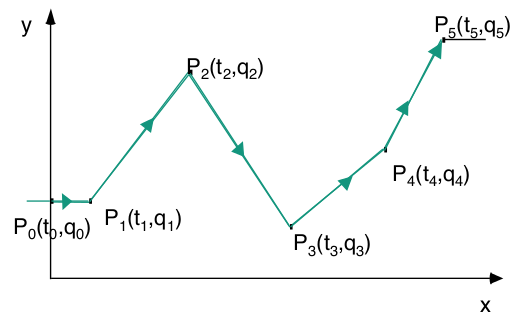
\includegraphics[scale=0.35]{graphics/linearinterpolation.png}
\caption{\label{fig:linearinterpolation} Beispiel der Linearinterpolation Quelle: \citep{rob1}}
\end{figure}
 Die Zirkularinterpolation schafft hingegen kreisförmige Verfahrwege zwischen zwei Punkte. Wenn man hingegen  Segmentweise interpoliert, werden die Endbedingungen der Teiltrajektorie i-1 und die Anfangsbedingungen der Teiltrajektorie i aneinander angepasst, so dass die Teiltrajektorien durch Splines beschrieben werden wie man auf der Abbildung \ref{fig:segmentinterpolation} sehen kann.
 \begin{figure}[h]
\center
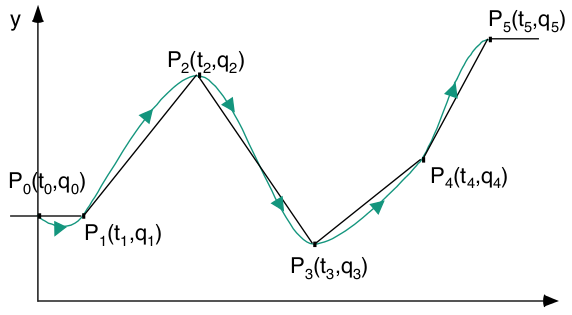
\includegraphics[scale=0.35]{graphics/segmentinterpolation.png}
\caption{\label{fig:segmentinterpolation} Beispiel der Segmentweise Bahninterpolation Quelle: \citep{rob1}}
\end{figure}
 
 
 Bei der approximative Bahnsteuerung werden anders als bei der Bahninterpolation, nicht alle Kontrollpunkte der Trajektorie befahren, sondern die Kontrollpunkte beeinflussen den Bahnverlauf und werden approximiert. Neben Bernsteinpolynome werden hier besonders Überschleifen benutzt um sanft Kurven zu fahren wie man auf der Abbildung \ref{fig:ueberschleifeninterpolation} sieht. Letzteres wurde auch in Praktikum eingesetzt.
 \begin{figure}[h]
\center
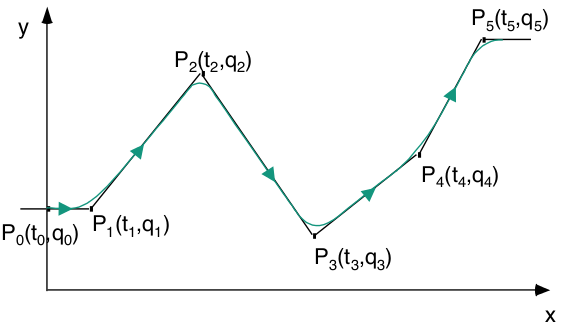
\includegraphics[scale=0.35]{graphics/ueberschleifeninterpolation.png}
\caption{\label{fig:ueberschleifeninterpolation} Beispiel der approximierte Bahnsteuerung mit Überschleifen Quelle: \citep{rob1}}
\end{figure}



% ********************************************************************************
% 										Umsetzung
% ********************************************************************************
\section{Umsetzung}
\label{bahnplanung_umsetzung_sec}


% -----------------------------------------------------------------------------
%													LowLevel-Ansteuerung
\subsection{LowLevel-Ansteuerung}
\label{bahnplanung_lowlevel_subsec}
\authorsection{\editoroier}

\todo[inline]{Oier: Schreiben}

% evtl. auch so ein Diagramm wie Abb. 4.4 von WS10/11?
%		bzw. Abb. 2.3 von WS09/10


% -----------------------------------------------------------------------------
%													Inverse Kinematik
\subsection{Inverse Kinematik}
\label{inverse_kinematik_subsec}
\authorsection{\editorjulian}

\todo[inline]{Julian: Schreiben}


% -----------------------------------------------------------------------------
%													Bahnplanung
\subsection{Bahnplanung}
\label{bahnplanung_subsec}
\authorsection{\editortobias}
\todo[inline]{Tobi: Schreiben}


\begin{itemize}
	\item Kurzer Grobüberblick über die Behaviours-Gruppe, hier werden Bahnplanungs-Aufgaben bearbeitet\todoprivate{ref zu behaviours-Bild}
	\begin{itemize}
		\item Berechnung von Trajektorien-Punkten auf Basis der Mensch-Position und Geschwindigkeit (Kinect)
		\item Schätzung der zukünftigen Position des Menschen
		\item Transformation von Welt- in Roboter- bzw. Bildkoordinaten und zurück\todoprivate{evtl. auch weg lassen}
		\item Abspeichern von Pfaden
		\item Abfahren von Pfaden
	\end{itemize}
	\item Module werden im Folgenden kurz beschrieben
	\item Kollisionsvermeidung als eigener Abschnitt
\end{itemize}

\missingfigure[figwidth=0.7\textwidth]{Behaviours}


\subsubsection{Position des Menschen}

\begin{itemize}
    \item bekommt aktuelle Position und Geschwindigkeit des Menschen von Kinect
    \item schätzt die zukünftige Position des Menschen anhand dieser Daten
    \item gibt aktuelle und geschätzte Position des Menschen aus
    \item Zeit-Parameter für die Schätzung: $t_{est}$
    \item Berechnung nach der Formel: $s_{est} = s_{act} + v \cdot t_{est}$
\end{itemize}


\subsubsection{Berechnung der Trajektorie}

\begin{itemize}
	\item Struktur der zu berechnenden Trajektorie duch \lstinline{OmniDriveAlongPath} \todoprivate{ref zu LowLevel?}\ vorgegeben:
	\begin{itemize}
		\item Start $(x,y)$, Koordinaten
		\item Following $(x,y,yaw)$, Koordinaten und Orientierung \todoprivate{Skizze zu x-y-z-roll-pitch-yaw ?}
		\item Next $(x,y)$, Koordinaten
	\end{itemize}
	\item Modul bekommt aktuelle und geschätzte Position des Menschen, sowie aktuelle Position des Roboters
	\item Berechnung einer neuen Trajektorie, sobald neue Mensch-Daten vorliegen
	\item Berechnung der Trajektorien-Punkte im Einzelnen:
	\begin{itemize}
	  \item Start: aktuelle Roboterposition
	  \item Next: Pose auf Roboter-Mensch-Vektor, die sich im Abstand $d$ vor dem Mensch befindet; yaw wird gesondert berechnet, sodass Roboter immer zu Mensch schaut
	  \item Following: Position auf next-estimated-Vektor, die sich $d$ vor geschätzter Mensch-Position befindet
	  \item erfolgt alles in absoluten Weltkoordinaten
  \end{itemize}
  \item Parameter $d$ für den Abstand des Roboters zum Menschen, default: $2m$
  \item Berechnung des yaw-Wertes: \todoprivate{Formel dazu}

% 	\item MUX für Trajektorie
% 	\begin{itemize}
% 		\item GenerateTrajectory
% 		\item LoadFromFile
% 	\end{itemize}
\end{itemize}

\todoprivate{Zeichnung mit Vektoren}



\subsubsection{Pfadspeichern und -laden}

\begin{itemize}
  \item Im \lstinline{followPerson} -Zustand: Wegpunkte $(x,y,yaw)$ werden in gewissen Abständen $d_{save}$ gespeichert
  \begin{itemize}
    \item sobald $ \overline{ s_{act} - s_{last} } > d_{save} $ \todoprivate{Fehler im Code??? Euklidischer Abstand stattdessen verwenden?}
  \end{itemize}
	\item Im \lstinline{loadPath} -Zustand: Nächster Wegpunkt wird geladen, sobald vorheriger erreicht wurde
  \begin{itemize}
		\item Im \lstinline{returnHome} -Zustand: Nächster Wegpunkt wird geladen, sobald vorheriger erreicht wurde; umgekehrte Reihenfolge
    \item sobald $ d( s_{foll} - s_{act} ) > d( s_{nxt} - s_{act} ) $, Euklidischer Abstand
  	\item \lstinline{yaw} wird unabhängig von Datei berechnet, sodass Roboter immer Menschen anschaut
  \end{itemize}
  \item Eigene Klasse zum File-Handling: \lstinline{fileUtil}
  \begin{itemize}
    \item Mehrere dump-files möglich
    \item Auslesen der Wegpunkte in normaler und umgekehrter Reihenfolge
  \end{itemize}
\end{itemize}



% 
% % -----------------------------------------------------------------------------
% %													Transformationen
% \subsection{Transformationen}
% \label{transformationen_subsec}
% 
% \authorsection{\editorjulian}
% \todo[inline]{Julian: Sollen wir (also du ;-) ) noch so einen Abschnitt machen?}


% -----------------------------------------------------------------------------
%													Kollisionsvermeidung
\subsection{Kollisionsvermeidung}
\label{kollisionsvermeidung_subsec}

\subsubsection{Modul}
\authorsection{\editortobias}
\todo[inline]{Tobi: Schreiben}

\begin{itemize}
 
  \item Kollisionsvermeidungsmodul (\lstinline{ObstacleAvoidance}) überprüft die geplante Trajektorie auf Hindernisse, und plant ggf. um Hindernisse
  \item Ausgaben von \lstinline{GenerateTrajectory} und \lstinline{LoadFromFile} werden geMUXt
  \begin{itemize}
    \item je nach Modus (\lstinline{followPerson} bzw. \lstinline{returnHome} / \lstinline{followPath}) schaltet MUX andere Eingänge durch
  	\item Die Ausgabe des MUX wird dann widerum komplett durch das Kollisionsvermeidungsmodul (\lstinline{ObstacleAvoidance}) geschleift
    \item Dadurch wird jede Trajektorie auf Hindernisse überprüft, keine kommt \glqq daran vorbei\grqq
  \end{itemize}
  \item Innerhalb des Moduls wird jede Trajektorie auf Hindernisse überprüft
	\begin{itemize}
	  \item die (Bild-)Punkte zwischen start, next und following werden berechnet (Transformation der Welt- in Bildkoordinaten)
	  \item Überprüfung für jeden einzelnen Punkt, ob er innerhalb eines Hindernisses liegt
	  \item Verwendung der \lstinline{ObstacleMap} \todoprivate{ref zu Lokalisierung}
	\end{itemize}
  \item Ohne Hindernis werden Trajektorien-Punkte nur durchgeschleift
  \item Wenn Hindernis erkannt, dann wird eine neue Trajektorie ermittelt
  \begin{itemize}
    \item Verwendung des A*-Algorithmus
    \item Ermittlung des Start- und Endpunktes für A*
    \item ggf. gesonderte Behandlung für Endpunkt (\lstinline{choosePointAfterObstacle})
    \item Aufruf A*
    \item Transformation der nuen Trajektorie IK $\rightarrow$ WK
  \end{itemize}

\end{itemize}



\subsubsection{Algorithmen}
\authorsection{\editorjulian}
\todo[inline]{Julian: Schreiben}

\begin{itemize}
	\item Überblick Planungsalgorithmen, Graphen, etc...
	\begin{itemize}
		\item A*
		\item D*
		\item Wavefront
		\item RRT
	\end{itemize}
	\item eventuell Tabelle mit kurzer Gegenüberstellung bzgl. Komplexität, Optimaliät des Pfades, Passend für unsere Aufgabe
	\item Am häufig verwendete Algorithmen
	\item state of the art
	\item Umsetzung des A*
\end{itemize}

% -----------------------------------------------------------------------------
%													Simulation
\subsection{Simulation}
\label{simulation_subsec}
\authorsection{\editoroier}
\todo[inline]{Oier: Schreiben}
